\documentclass[class=article, crop=false]{standalone}

\begin{document}
\section*{Partie 1 - Equation de Lagrange}
\paragraph{Présentation}Ce Travail Pratique évaluera la capacité d'entant donné une système le modéliser, le proposer un contrôleur et un observateur et, à la fin, les intégrées. Pendant ce development, des simulations MATLAB et Simulink seront proposées pour valider le development et permettre de visualiser les résultats.

\paragraph{Résultats}Comme le but de ce travail est la modélisation du système le development des equations qui décrivent le système seront déjà connus. Sur ce Travail Pratique les Questions 1, 2 et 3 ont les résultats nécessaires pour le déroulement du projet et seront rappelles à la suite.

\paragraph{Problème}On s'intéresse à la stabilisation d'une balle libre de rouler sur un plateau pivotant comme montrer dans la figure suivante:
\begin{figure}[H]
    \centering
    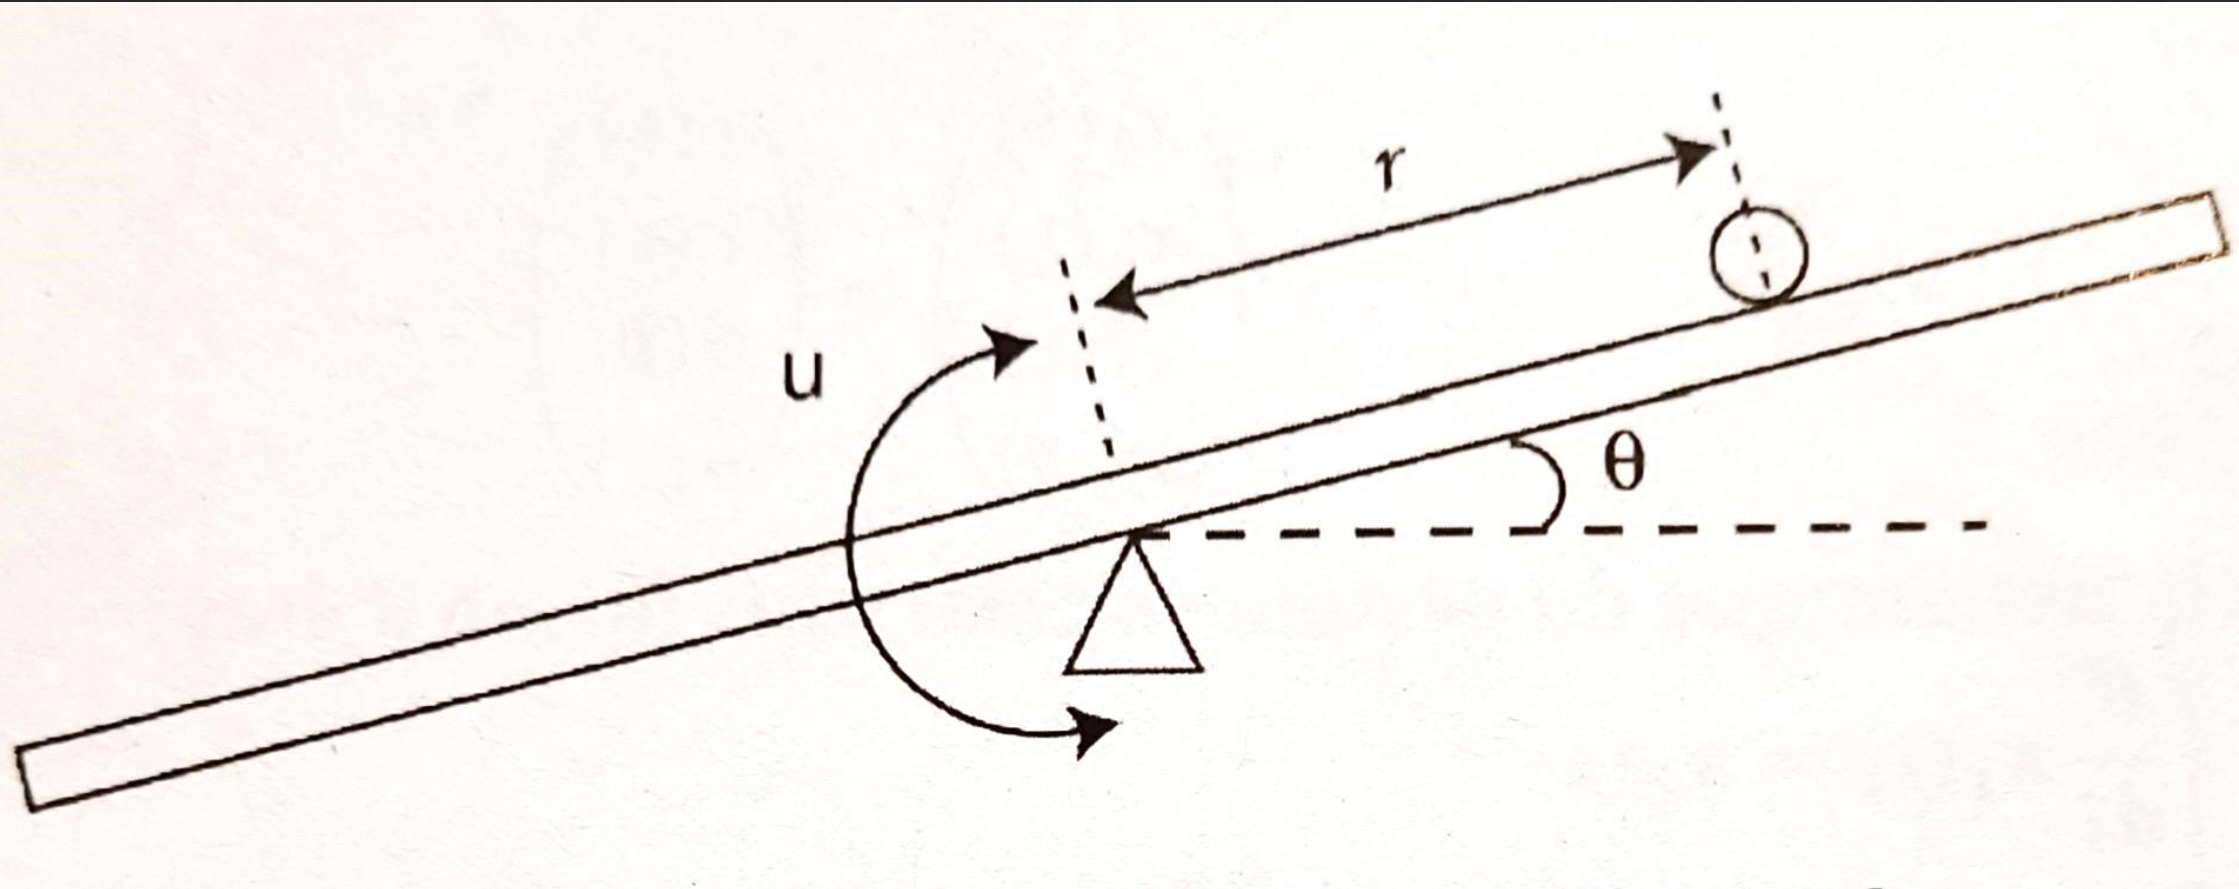
\includegraphics[height = 40mm]{../images/system.png}
    \caption{Système d'Intéresse}
    \label{fig:system}
\end{figure}
Où:
\begin{enumerate}[noitemsep, rightmargin = \leftmargin]
    \item $J_p$, \textbf{Moment d'Inertie du Plateau} par rapport à on axe de rotation;
    \item $J_b$, \textbf{Moment d'Inertie de la Balle} par rapport à son centre;
    \begin{equation}\label{eq:def_Jb}
        J_b = \sigma \cdot m \cdot R^2,
        \qquad
        0 < \sigma \leq 1
    \end{equation}
    Où:
    \begin{enumerate}[noitemsep, rightmargin = \leftmargin]
        \item $\sigma$, \texttt{Densité} en fonction du rayon;
    \end{enumerate}

    \item $R$, \textbf{Rayon de la Balle};
    \item $m$, \textbf{Masse de la Balle};
    \item $g$, \textbf{Accélération Gravitationnelle};
\end{enumerate}
Avec:
\begin{enumerate}[noitemsep, rightmargin = \leftmargin]
    \item $r(t)$, \textbf{Distance de la Balle} par rapport au Centre du Plateau sur le temps;
    \item $\theta(t)$, \textbf{Angle du Plateau} par rapport son Centre de Rotation sur le temps;
    \item $u(t)$, \textbf{Commande du Système};
\end{enumerate}
On souhaite maintenir la Balle sur la position $r_{\text{ref}}$ à partir des données obtenus des capteurs $r(t)$ et $\theta(t)$ en utilisant la commande $u(t)$ qui contrôle l'angle du Plateau.
\begin{remark}
    Même que le document utilisé barre et balle pour nommer les partis du système, on appellera la barre comme plateau pour que les sous-écrits soit différent en facilitant la comprehension de la résolution.
\end{remark}
\begin{remark}
    On considère que les angles de commande seront petits car la puissance disponibles pour la commande sont petits.
\end{remark}

\subsection*{Question 1}
\begin{exercise}
    Montrer que l'énergie cinétique du système est donne par:
    \begin{equation}\label{eq:def_Ec}
        \boxed{
            E_c = 
            \frac{1}{2} \cdot J_p \cdot \dot{\theta}^2(t) +
            \frac{1}{2} \cdot m \cdot (\dot{r}^2(t) + r^2(t) \cdot \dot{\theta}^2(t)) +
            \frac{1}{2} \cdot J_b \cdot \frac{\dot{r}^2}{R^2}
        }
    \end{equation}
    \begin{remark}
        On négligera dans l'énergie cinétique de rotation de la balle sur elle-même, c'est-à-dire: l'effet de la rotation de la barre $\dot{\theta}(t)$.
    \end{remark}
\end{exercise}

\subsection*{Question 2}
\begin{exercise}
    Calculer l'énergie potentielle $E_p$ en fonction de $r(t)$ e $\theta(t)$.

    \begin{remark}
        On supposera que l'axe de rotation est au niveau du centre de gravité du plateau.
    \end{remark}
\end{exercise}
\begin{resolution}
    L'Énergie Potentielle sera donne par l'équation suivante:
    \begin{equation}\label{eq:def_Ep}
        \boxed{
            E_p = m \cdot g \cdot r \cdot \sin(\theta(t))
        }
    \end{equation}
\end{resolution}

\subsection*{Question 3}
\begin{exercise}
    Déduire de ce qui précède les équations de Lagrange suivantes:
    \begin{align}
        (1 + \sigma) \cdot \frac{\text{d}}{\text{dt}} \dot{r}(t) 
        &= 
        r(t) \cdot \dot{\theta}^2(t) - g \cdot \sin(\theta(t))
        \label{eq:def_Lagrange1}\\
        \frac{\text{d}}{\text{dt}} (J_p + m \cdot r^2(t)) \cdot \dot{\theta}(t)
        &= 
        -m \cdot g \cdot r(t) \cdot \cos(\theta(t)) + u(t)
        \label{eq:def_Lagrange2}
    \end{align}
\end{exercise}
\end{document}